\documentclass{standalone}

\begin{document}

\subsection[Synapse]{Synapse dataset}\label{synapse:synapse}

As benchmark dataset was chosen the core sets extracted from the The Cancer Genome Atlas (accession number \href{https://www.synapse.org/#!Synapse:syn300013/wiki/27406}{syn300013, doi:10.7303/syn300013}) (\emph{Synapse dataset} in the following), used in a previous study~\cite{Yuan2014} which aimed at quantifying the role of different omics data types (e.g. mRNA and miRNA microarray data,  protein levels measured with Reverse Phase Protein Array - RPPA) via different state-of-the-art classification methods.
This allowed us to compare our results to a large set of commonly used classification methods, by using their performance validation pipeline (accession number \href{https://www.synapse.org/#!Synapse:syn1710282/wiki/27303}{syn1710282, doi:10.7303/syn1710282}).

The Synapse dataset is composed by four tumors datasets: kidney renal clear cell carcinoma (KIRC), glioblastoma multiforme (GBM), ovarian serous cystadenocarcinoma (OV) and lung squamous cell carcinoma (LUSC).
For each cancer type we applied the DNetPRO algorithm on mRNA, miRNA and RPPA data and we compare the performances results with the Yuan et al. ones.

The summary description of the datasets used is reported in the Tab.~\ref{tab:synapse}.

\begin{table}[htbp]
\centering
\begin{tabular}{lccccccc}
\hline \rowcolor{darkgrayrow}
         &               &                &          & Number       \\
\rowcolor{darkgrayrow}
Cancer   & mRNA          & miRNA          & Protein  & of samples   \\
\hline
GBM      & AgilentG4502A & H-miRNA\_8x15k & RPPA     &              \\
         & 17814         & 533            & $^a$     & 210          \\
KIRC     & HiseV2        & GA+Hiseq       & RPPA                    \\
         & 20530         & 1045           & 166      & 243          \\
OV       & AgilentG4502A & H-miRNA\_8x15k & RPPA     &              \\
         & 17814         & 798            & 165      & 379          \\
LUSC     & HiseqV2       & GA+Hiseq       & RPPA     &              \\
         & 20530         & 1045           & 174      & 121          \\
\hline
\end{tabular}
\caption{In the first row platforms are reported and the second shows the dimension of dataset as number of probes.
AgilentG4502A: Agilent 244K Custom Gene Expression G4502A;
HiseqV2: Illumina HiSeq 2000 RNA Sequencing V2;
H-miRNA\_8x15K: Agilent 8~×~15K Human miRNA-specific microarray platform;
GA+Hiseq: Illumina Genome Analyzer/HiSeq 2000 miRNA sequencing platform;
RPPA: MD Anderson reverse phase protein array.
The last column shows the number of sample.
\newline $^a$ Missing data-type for that cancer type.
}
\label{tab:synapse}
\end{table}

Each tumor dataset was pre-processed by adding a zero-mean Gaussian random noise ($\sigma = 10^{-4}$)) to remove the possible null values in the database, which could produce numerical errors in the distances evaluation between genes.
Then, we randomly split each dataset in training and test sets with a stratified (i.e. balanced for class sample ratio) 10-fold procedure: with the stratification we are reasonably sure that each training-set is a good representative of the whole sample set.
The choice of a 10-fold splitting is aimed to reproduce the analysis pipeline presented by Yuan et al. with an analogous cross-validation procedure.
Since we don't have exact details of their data splitting, the cross validation was repeated 100 times, for a total of 1000 training procedures for each tumor (OV, LUSC, KIRC, GB) and data type (mRNA, miRNA, RPPA).
Each training procedure led to the extraction of multiple signatures.

We chose threshold values in order to obtain a resulting number of variables (network nodes) in the order of $10^2-10^3$, and identified all connected components of the network as signatures.
If more than one component existed, each one was considered as a different signature.

The final multidimensional signatures were tested by a Discriminant Analysis with a diag-quadratic distance, to avoid possible problems about covariance matrix inversion (as for the Mahalanobis distance).

\begin{center}
\begin{figure}[htbp]
\centering
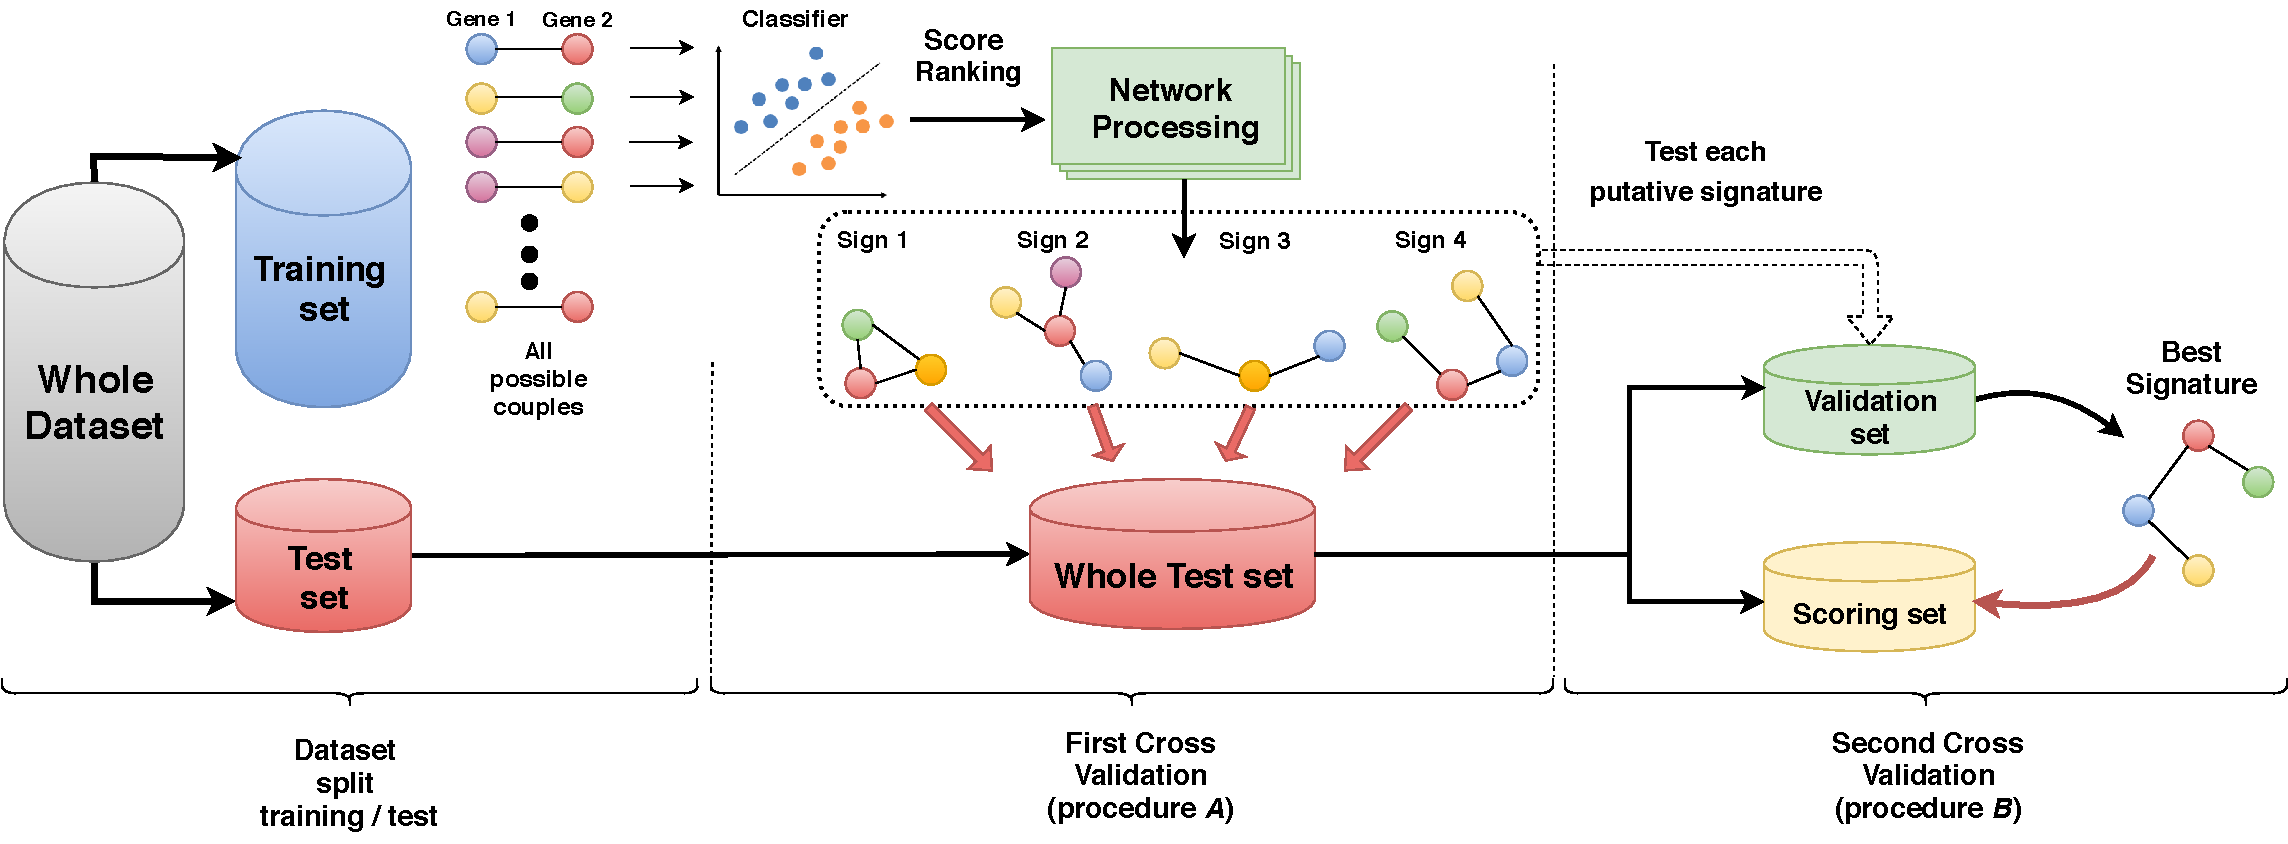
\includegraphics[width=1.0\textwidth]{dnet_pipe.pdf}
\caption{Scheme of DNetPRO algorithm.
On the \quotes{training set}, all possible couples of variables are used for Discriminant Analysis, generating the fully connected network weighted by classification performance.
Thresholding ranked couples, several signatures can result (as connected components) and their performance is evaluated on the \quotes{whole test set} (procedure $A$).
% Signatures are given by the connected components created by all couples with scorer greater than a chosen threshold.
A unique best signature can be identified on a \quotes{validation set} and tested in a \quotes{scoring set}, obtained by further splitting the \quotes{whole test set} (procedure $B$).
% The pipeline parameters was adapted to faithfully mimic the reference work-flow to allow a comparison of the final results except for the second cross validation step.
}
\label{fig:dnet_pipe}
\end{figure}
\end{center}

We remark that DNetPRO can provide more than one signature as a final outcome, given by all the connected components found in the variable network, or a unique top-performing signature can be obtained by a further cross-validation step (procedure $A$ and procedure $B$ in Fig.~\ref{fig:dnet_pipe}, respectively).

In the single cross validation configuration (procedure $A$ in Fig.~\ref{fig:dnet_pipe}), the best signature was extracted as the one reaching the highest accuracy score during the training step.
This best signature was then tested over the available test set.

When also the second cross validation was used (procedure $B$ in Fig.~\ref{fig:dnet_pipe}) the best signature wasted as the most performing over a subset of the whole test set (\emph{validation set}), and the final performance was evaluated on the remaining \emph{scoring set}.

To compare our results with the work of Yuan et al., we used the AUC (\emph{Area Under the Curve}) score, that they provided in the paper as the result of their analyses.
The distribution of our results could be compared to the single score value given in the other work.

\end{document}
